\section{$\mathcal{H}_\infty$ Design}
The linearized model in \autoref{sec:linearizationModel} has varying parameters, such as the added mass and damping coefficients. The vessel may also experience external disturbances, such as wind forces. During surveying, the vessel needs to be robust to these model variations and it must be able to sufficiently reject disturbances. Using the $\mathcal{H}_\infty$ design technique, a robust controller for the vessel can be synthesized.

\subsection{$\mathcal{H}_\infty$ State Space Model}
The state space model from \autoref{xDotLinear} and \autoref{yLinear} needs to be remodeled into a state space form suitable for the $\mathcal{H}_\infty$ controller design. This representation starts with the equations
\begin{flalign}
  \vec{\dot{x}}(t) &= \vec{A_1} \vec{x}(t) + \vec{B_1} \vec{w}(t) + \vec{B_2} \vec{u}(t)\ ,
  \label{xDotLinearH} \\
  \vec{z}(t) &= \vec{C_1} \vec{x}(t) + \vec{D_{11}} \vec{w}(t) + \vec{D_{12}} \vec{u}(t)\ ,
  \label{xDotLinearH} \\
  \vec{y}(t) &= \vec{C_2} \vec{x}(t) + \vec{D_{21}} \vec{w}(t) + \vec{D_{22}} \vec{u}(t)\ ,
  \label{yLinear} 
\end{flalign}
\begin{where}
  \va{\vec{x}}{is the state vector}{}
  \va{\vec{w}}{is the uncontrolled input vector}{}
  \va{\vec{u}}{is the controlled input vector}{}
  \va{\vec{z}}{is the performance output vector}{}
  \va{\vec{y}}{is the measured output vector}{}
  \va{\vec{A_1}}{is the state matrix}{}
  \va{\vec{B_1}}{is the uncontrolled input matrix}{}
  \va{\vec{B_2}}{is the controlled input matrix}{}
  \va{\vec{C_1}}{is the performance output matrix}{}
  \va{\vec{D_{11}}}{is the direct feedthrough matrix from $\vec{w}$ to $\vec{z}$}{}
  \va{\vec{D_{12}}}{is the direct feedthrough matrix from $\vec{u}$ to $\vec{z}$}{}
  \va{\vec{C_2}}{is the output matrix}{}
  \va{\vec{D_{21}}}{is the direct feedthrouhg matrix from $\vec{w}$ to $\vec{y}$}{}
  \va{\vec{D_{22}}}{is the direct feedthrouhg matrix from $\vec{u}$ to $\vec{y}$}{}
\end{where}

The $\mathcal{H}_\infty$ model representation can also be seen in \autoref{fig:HinfDiag}, where all signals and matrices involved on the design process are represented.
\begin{figure}[H]
	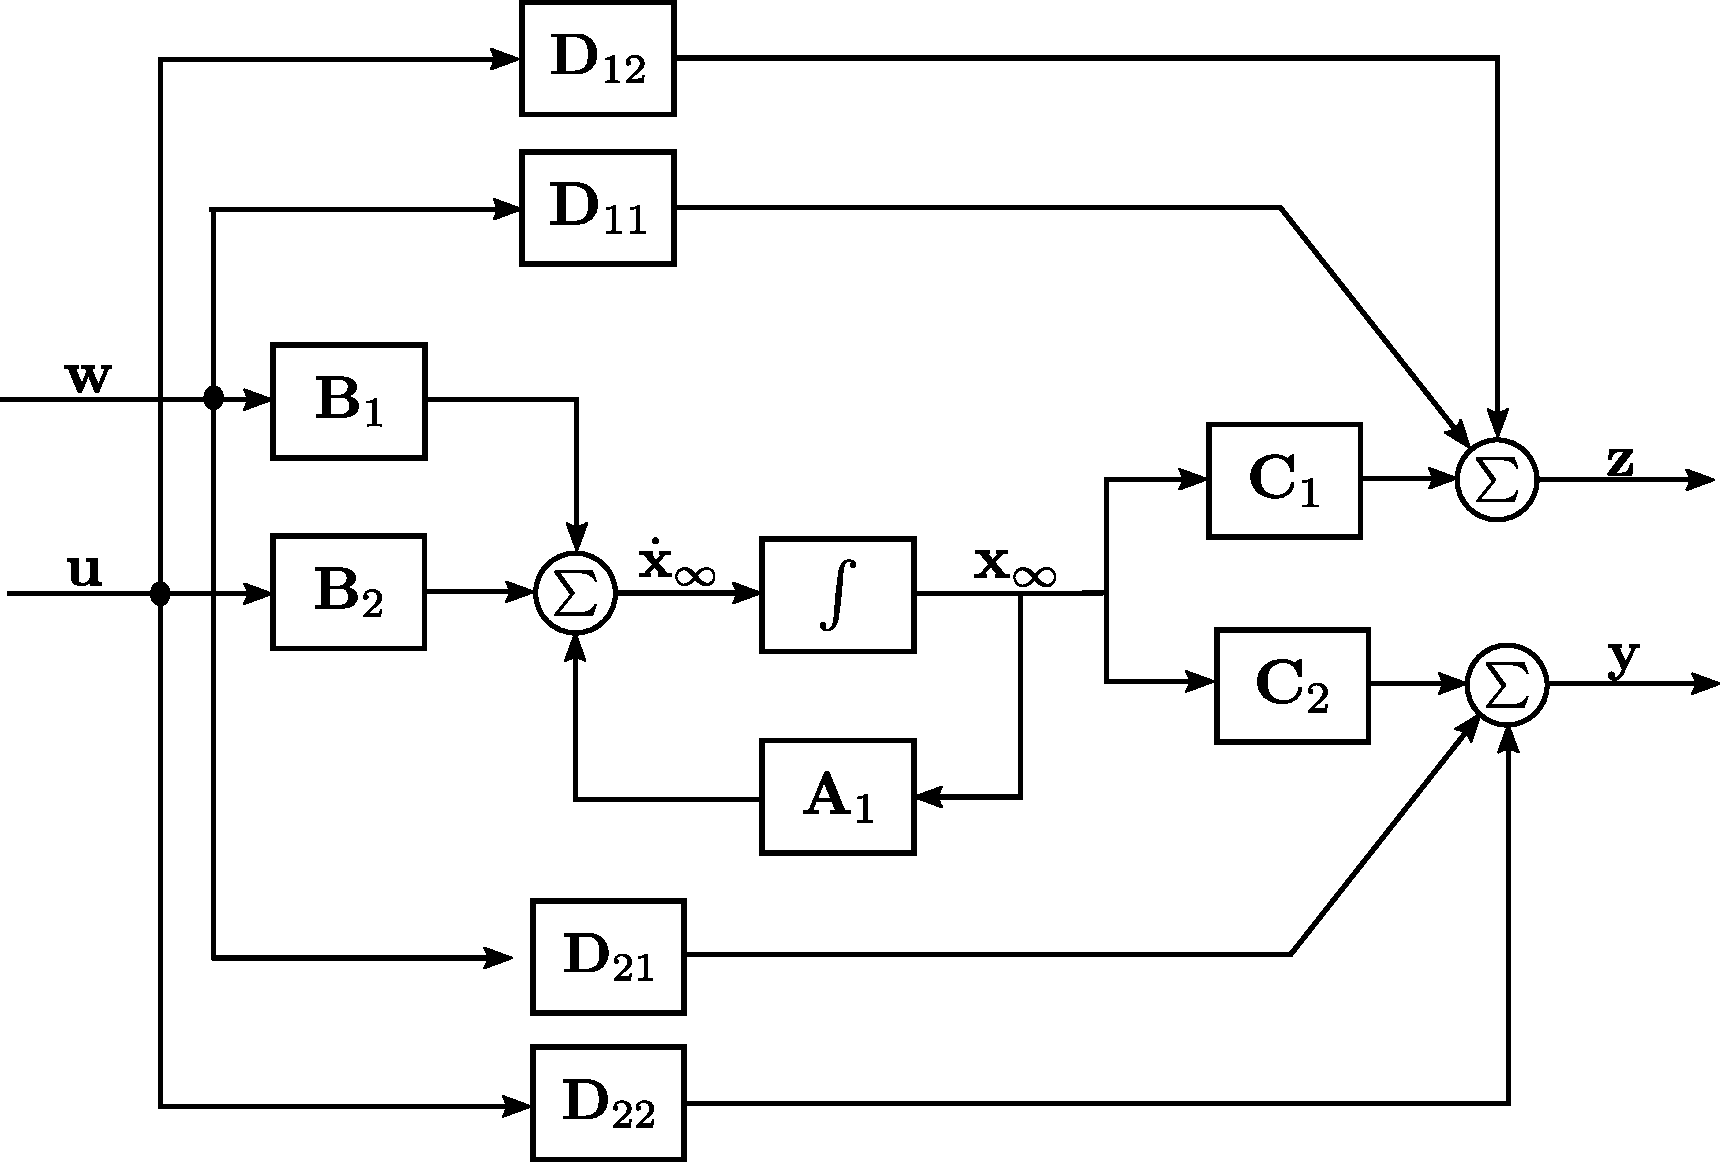
\includegraphics[width=0.6\textwidth]{figures/HinfDiag}
	\caption{Block diagram used in the $\mathcal{H}_\infty$ controller design.}
	\label{fig:HinfDiag}
\end{figure}
